%!TeX root=Hauptdokument.tex
\chapter{Hauptteil}

\blindtext[1]

\blindtext[2]

\blindtext[2]

\blindtext[2]

% Float Objekte
\begin{figure}
\centering
\fbox{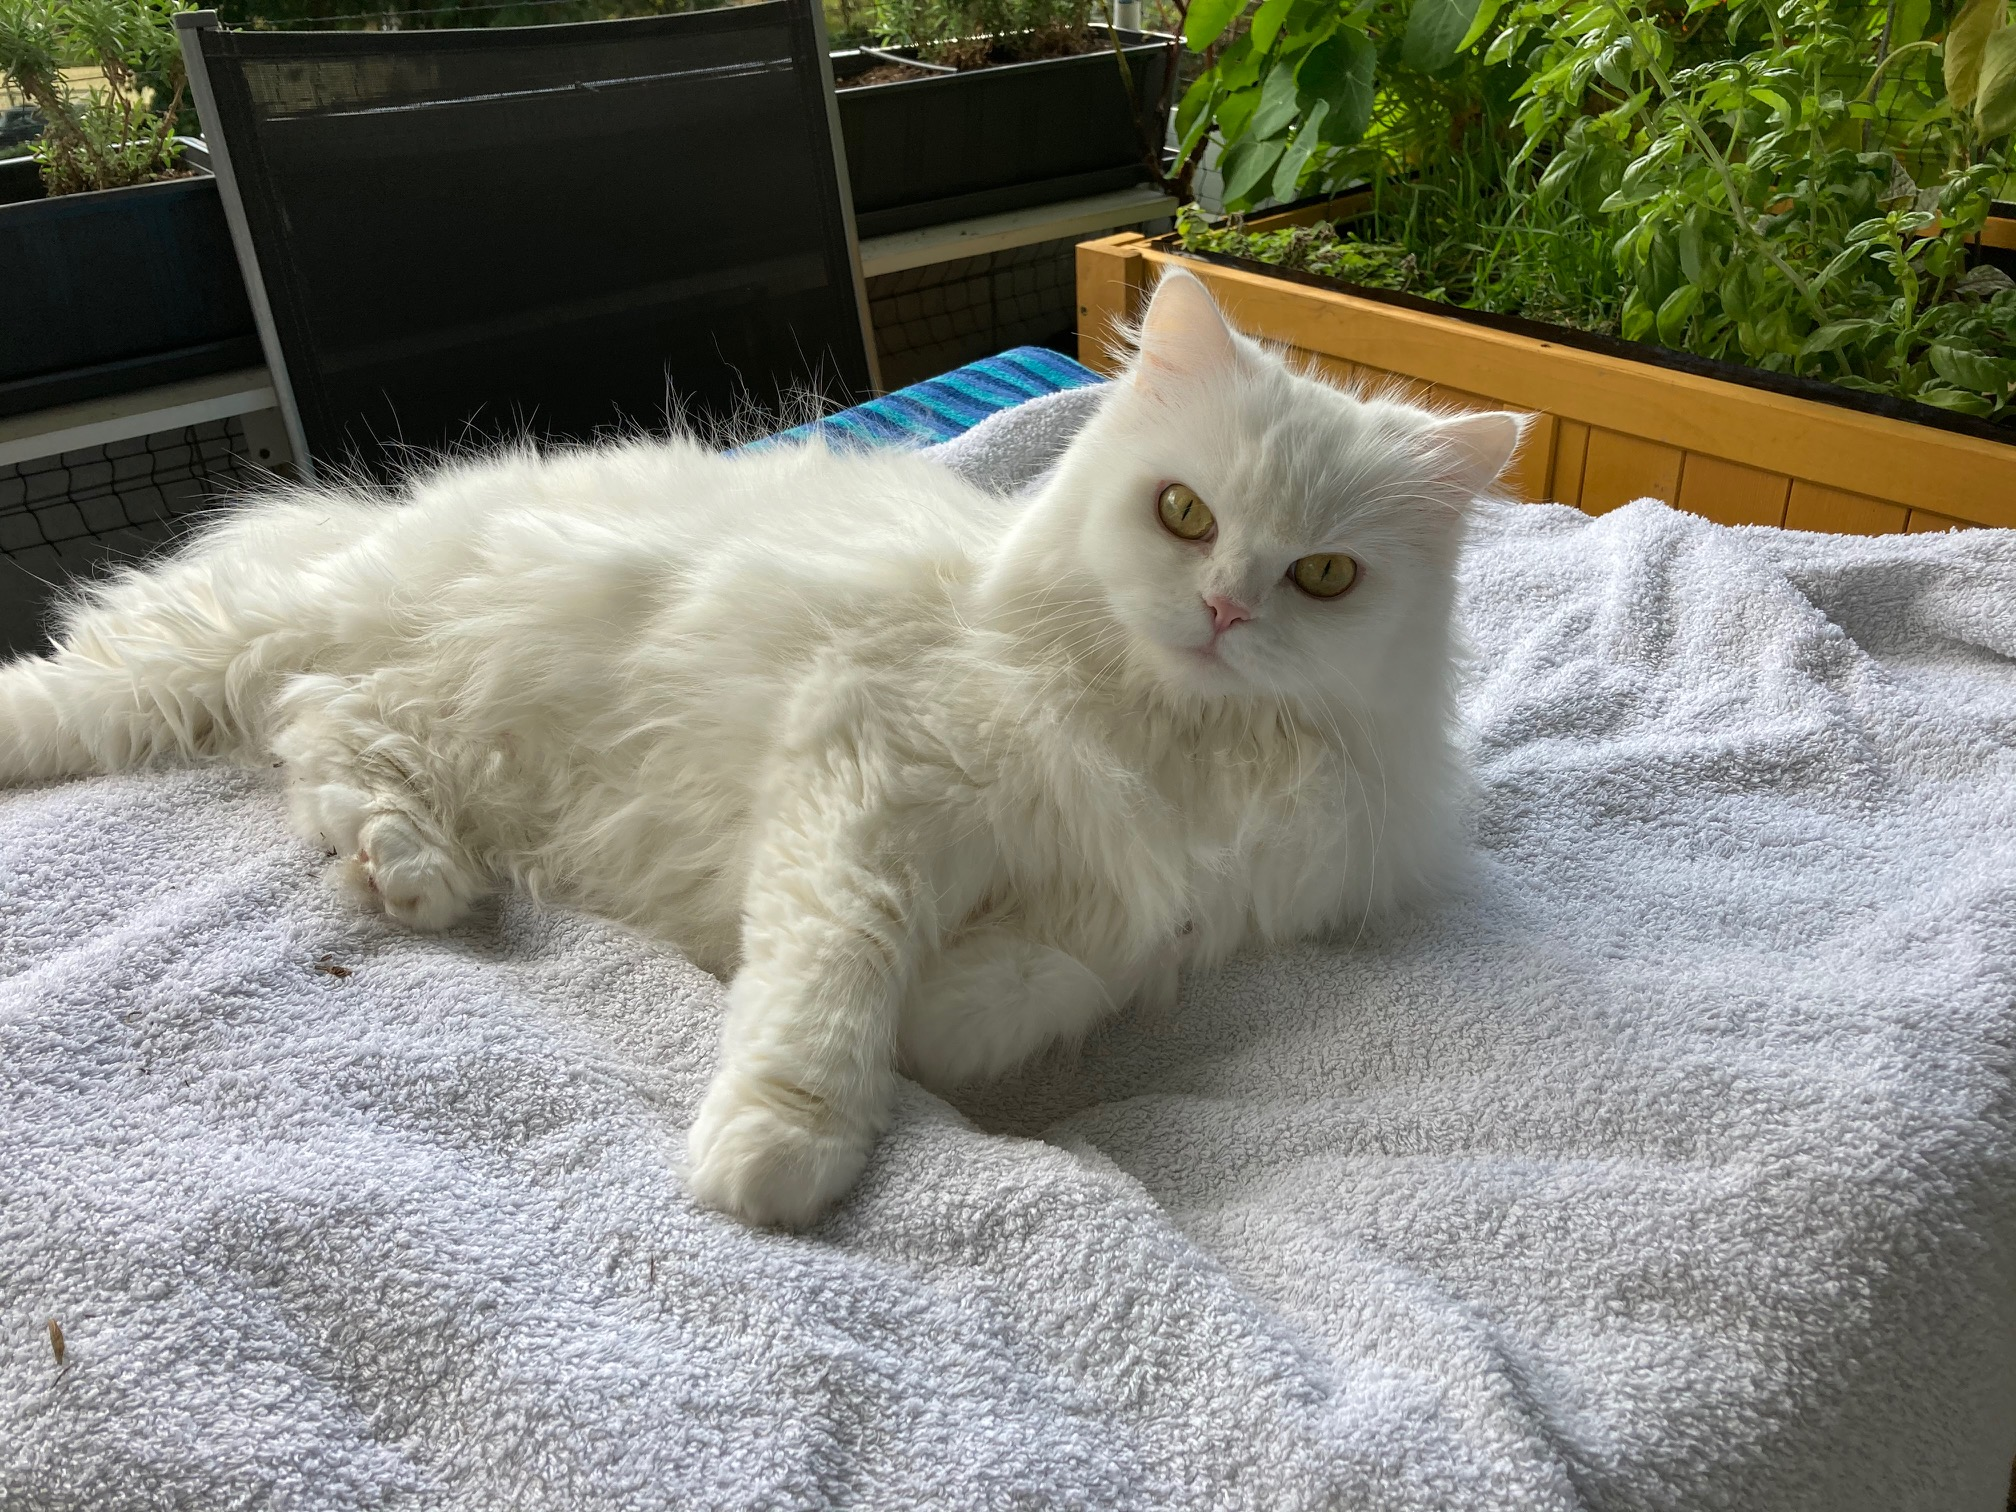
\includegraphics[width=0.75\textwidth]{../Bilder/Katze1}}
\caption{Meine Katze}\label{fig:katze1}
\end{figure}

% Float Objekte
\begin{figure}
\centering
\fbox{
\includegraphics[width=0.75\textwidth]{../Bilder/Katze2}}
\caption{Meine Katze nochmal}\label{fig:katze2}
\end{figure}


\blindtext[2]

% Wenn ein Bild eine Unterschrift braucht, aber nicht ``floaten'' soll
% dann nimm \captionof{}{}
\begin{center}

\includegraphics[width=0.75\textwidth,angle=45]{../Bilder/Katze2}
\captionof{figure}{Meine Katze nochmal}\label{fig:katze3}
\end{center}


\blindtext[2]


\blindtext[2]

%Paket subcaption
\begin{figure}
\centering
\subcaptionbox{Eine Katze \label{cat1}}
{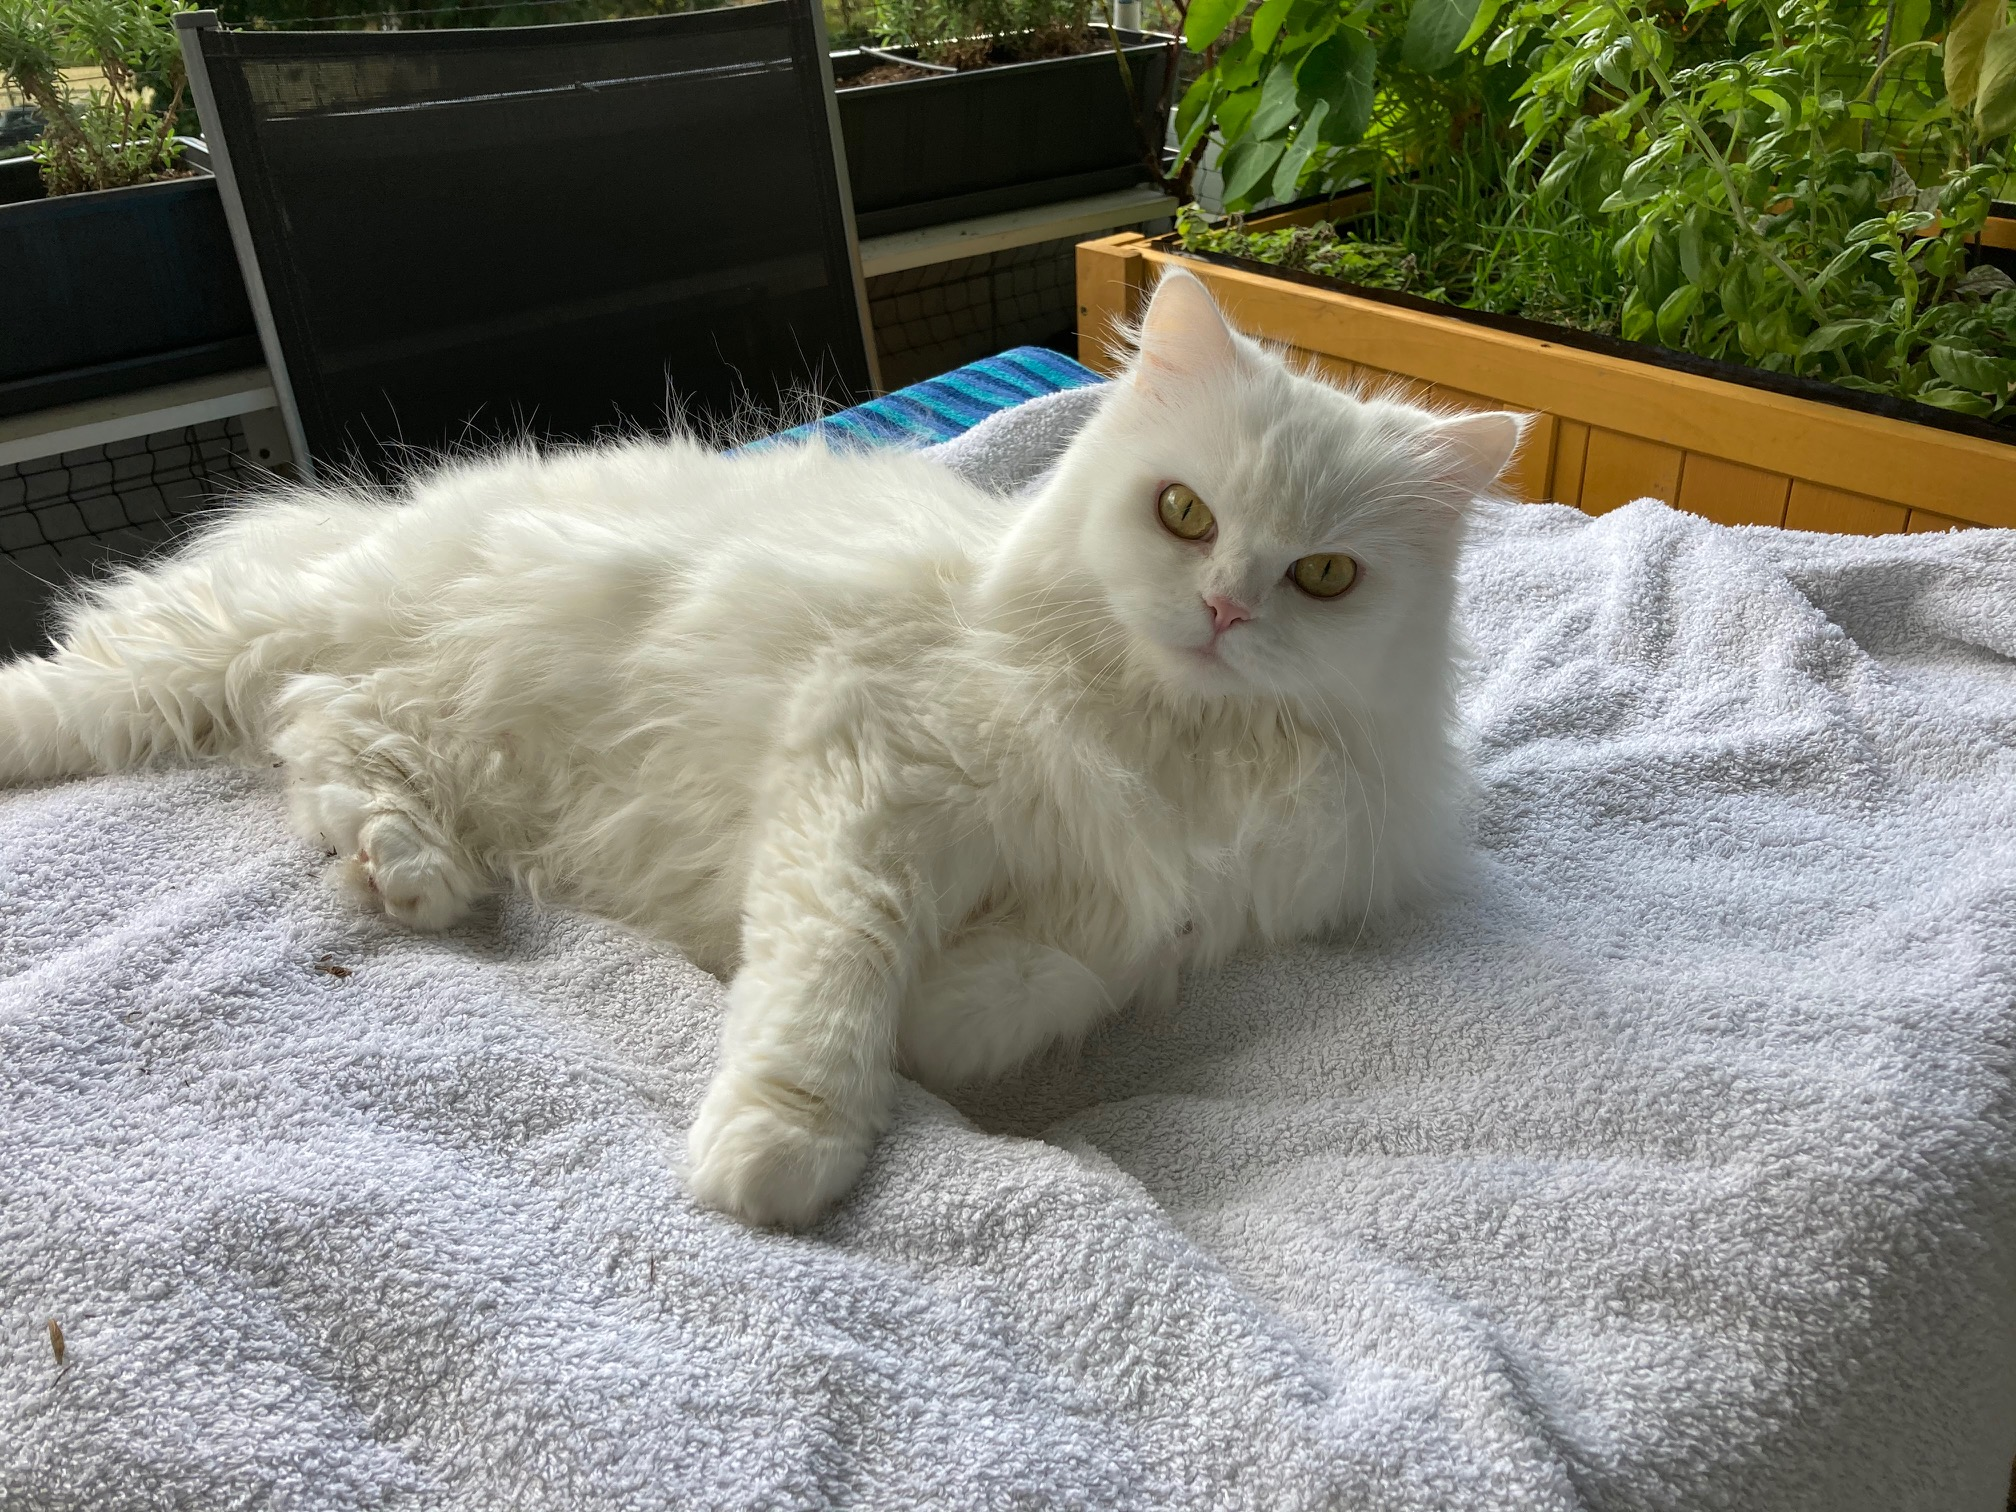
\includegraphics[width=0.49\textwidth]{../Bilder/Katze1}}
\subcaptionbox{Die selbe Katze \label{cat2}}
{
\includegraphics[width=0.49\textwidth]{../Bilder/Katze2}}
\caption{Zwei Katzenbilder}\label{katzenbilder}
\end{figure}






